% \documentclass[table]{beamer}
\documentclass[table,handout]{beamer}
\setbeameroption{show notes}
% \setbeameroption{hide notes}
% \setbeameroption{show only notes}
\usepackage{varwidth}

\newif\ifhide
\newif\ifpost
\newif\ifhideclicker

% \hidetrue
% \hideclickertrue
% \posttrue

\newcommand{\whiteout}[1]{\textcolor{white}{#1}}
% \newcommand{\whiteoutbox}[1]{\fcolorbox{white}{white}{\parbox{\dimexpr \linewidth-2\fboxsep-2\fboxrule}{\whiteout{#1}}}}
% \newcommand{\notebox}[1]{\fcolorbox{blue}{white}{\parbox{\dimexpr \linewidth-2\fboxsep-2\fboxrule}{#1}}}
\newcommand{\whiteoutbox}[1]{\fcolorbox{white}{white}{\parbox{\linewidth}{\whiteout{#1}}}}
\newcommand{\notebox}[1]{\fcolorbox{blue}{white}{\parbox{\linewidth}{#1}}}
\newcommand{\blankbox}[1]{\phantom{\varwidth{\linewidth}\whiteoutbox{#1}\endvarwidth}}
\newcommand{\blank}[1]{\phantom{\varwidth{\linewidth}#1\endvarwidth}}

\ifhide%
    \newcommand{\hmask}[1]{\blank{#1}}%
\else%
    \newcommand{\hmask}[1]{#1}%
\fi

\ifhide%
    \newcommand{\wout}[1]{\whiteout{#1}}%
\else%
    \newcommand{\wout}[1]{#1}%
\fi

\ifhide%
    \newcommand{\hignore}[1]{}%
\else%
    \newcommand{\hignore}[1]{#1}%
\fi

\ifpost%
    \newcommand{\nopost}[1]{}%
\else%
    \newcommand{\nopost}[1]{#1}%
\fi

\ifhideclicker%
    \newcommand{\clickerslide}[1]{\stepcounter{clickerQuestionCounter}%
        \begin{frame}[t]
            \textcolor{blue}{Q \arabic{clickerQuestionCounter}:}
        \end{frame}}
\else%
    \newcommand{\clickerslide}[1]{#1}%
\fi

\ifhide%
    \newcommand{\hidebox}[1]{\blank{#1}}%
\else%
    \newcommand{\hidebox}[1]{\notebox{#1}}%
\fi

\ifhide%
    \newcommand{\wbox}[1]{\whiteoutbox{#1}}%
\else%
    \newcommand{\wbox}[1]{\notebox{#1}}%
\fi

\ifhide%
    \newcommand{\nbox}[1]{\blankbox{#1}}%
\else%
    \newcommand{\nbox}[1]{\notebox{#1}}%
\fi

\ifhideclicker%
    \newcommand{\clickeranswer}[1]{#1}%
\else%
    \ifhide%
        \newcommand{\clickeranswer}[1]{#1}%
    \else%
        \newcommand{\clickeranswer}[1]{\textbf{\textcolor{blue}{#1}}}%
    \fi
\fi

\usepackage{beamerthemesplit}
% \usetheme{boxes}
\usetheme{Malmoe}
\usecolortheme{seahorse}
% \usecolortheme{seagull}
\usepackage{ifthen}
\usepackage{xspace}
\usepackage{multirow}
\usepackage{multicol}
\usepackage{booktabs}
\usepackage{xcolor}
\usepackage{wasysym}
\usepackage{comment}
\usepackage{hyperref}
\hypersetup{pdfborder={0 0 0}, colorlinks=true, urlcolor=blue, linkcolor=blue, citecolor=blue}
\usepackage{changepage}
\usepackage[compatibility=false]{caption}
\captionsetup[figure]{font=scriptsize, labelformat=empty, textformat=simple, justification=centering, skip=2pt}
\usepackage{tikz}
\usetikzlibrary{trees,calc,backgrounds}

\usepackage[bibstyle=joaks-slides,maxcitenames=3,mincitenames=1,backend=biber]{biblatex}

\newrobustcmd*{\shortfullcite}{\AtNextCite{\renewbibmacro{title}{}\renewbibmacro{in:}{}\renewbibmacro{number}{}}\fullcite}

\newrobustcmd*{\footlessfullcite}{\AtNextCite{\renewbibmacro{title}{}\renewbibmacro{in:}{}}\footfullcite}

% Make all footnotes smaller
% \renewcommand{\footnotesize}{\scriptsize}

\definecolor{myGray}{gray}{0.9}
\colorlet{rowred}{red!30!white}

\setbeamertemplate{blocks}[rounded][shadow=true]

\setbeamercolor{defaultcolor}{bg=structure!30!normal text.bg,fg=black}
\setbeamercolor{block body}{bg=structure!30!normal text.bg,fg=black}
\setbeamercolor{block title}{bg=structure!50!normal text.bg,fg=black}

\newenvironment<>{varblock}[2][\textwidth]{%
  \setlength{\textwidth}{#1}
  \begin{actionenv}#3%
    \def\insertblocktitle{#2}%
    \par%
    \usebeamertemplate{block begin}}
  {\par%
    \usebeamertemplate{block end}%
  \end{actionenv}}

\newenvironment{displaybox}[1][\textwidth]
{
    \centerline\bgroup\hfill
    \begin{beamerboxesrounded}[lower=defaultcolor,shadow=true,width=#1]{}
}
{
    \end{beamerboxesrounded}\hfill\egroup
}

\newenvironment{onlinebox}[1][4cm]
{
    \newbox\mybox
    \newdimen\myboxht
    \setbox\mybox\hbox\bgroup%
        \begin{beamerboxesrounded}[lower=defaultcolor,shadow=true,width=#1]{}
    \centering
}
{
    \end{beamerboxesrounded}\egroup
    \myboxht\ht\mybox
    \raisebox{-0.25\myboxht}{\usebox\mybox}\hspace{2pt}
}

\newenvironment{mydescription}{
    \begin{description}
        \setlength{\leftskip}{-1.5cm}}
    {\end{description}}

\newenvironment{myitemize}{
    \begin{itemize}
        \setlength{\leftskip}{-.3cm}}
    {\end{itemize}}

% footnote without a marker
\newcommand\barefootnote[1]{%
  \begingroup
  \renewcommand\thefootnote{}\footnote{#1}%
  \addtocounter{footnote}{-1}%
  \endgroup
}

% define formatting for footer
\newcommand{\myfootline}{%
    {\it
    \insertshorttitle
    \hspace*{\fill} 
    \insertshortauthor, \insertshortinstitute
    % \ifx\insertsubtitle\@empty\else, \insertshortsubtitle\fi
    \hspace*{\fill}
    \insertframenumber/\inserttotalframenumber}}

% set up footer
\setbeamertemplate{footline}{%
    \usebeamerfont{structure}
    \begin{beamercolorbox}[wd=\paperwidth,ht=2.25ex,dp=1ex]{frametitle}%
        % \Tiny\hspace*{4mm}\myfootline\hspace{4mm}
        \tiny\hspace*{4mm}\myfootline\hspace{4mm}
    \end{beamercolorbox}}

% remove navigation bar
\beamertemplatenavigationsymbolsempty

\makeatletter
    \newenvironment{noheadline}{
        \setbeamertemplate{headline}[default]
        \def\beamer@entrycode{\vspace*{-\headheight}}
    }{}
\makeatother

\newcounter{clickerQuestionCounter}
\ifhideclicker%
\newenvironment{clickerquestion}
{ \stepcounter{clickerQuestionCounter}
  \begin{enumerate}[Q \arabic{clickerQuestionCounter}:]\color{white} }
{ \end{enumerate} }
\else%
\newenvironment{clickerquestion}
{ \stepcounter{clickerQuestionCounter}
  \begin{enumerate}[Q \arabic{clickerQuestionCounter}:] }
{ \end{enumerate} }
\fi

\ifhideclicker%
\newenvironment{clickeroptions}
{ \begin{enumerate}[\begingroup\color{white} 1)\endgroup]\color{white} }
{ \end{enumerate} }
\else%
\newenvironment{clickeroptions}
{ \begin{enumerate}[\begingroup\color{red} 1)\endgroup] }
{ \end{enumerate} }
\fi


\tikzstyle{centered} = [align=center, text centered, font=\sffamily\bfseries]
\tikzstyle{skip} = [centered, inner sep=0pt, fill]
\tikzstyle{empty} = [centered, inner sep=0pt]
\tikzstyle{inode} = [centered, circle, minimum width=4pt, fill=black, inner sep=0pt]
\tikzstyle{tnode} = [centered, circle, inner sep=1pt]
\tikzset{
  % edge styles
  level distance=10mm,
  mate/.style={edge from parent/.style={draw,distance=3pt}},
  mleft/.style={grow=left, level distance=10mm, edge from parent path={(\tikzparentnode.west)--(\tikzchildnode.east)}},
  mright/.style={grow=right, level distance=10mm, edge from parent path={(\tikzparentnode.east)--(\tikzchildnode.west)}},
  % node styles
  male/.style={rectangle,minimum size=4mm,fill=gray!80},
  female/.style={circle,minimum size=4mm,fill=gray!80},
  amale/.style={male,fill=red},
  afemale/.style={female,fill=red},
}

\newcommand{\highlight}[1]{\textcolor{violet}{\textit{\textbf{#1}}}}
\newcommand{\super}[1]{\ensuremath{^{\textrm{\sffamily #1}}}}
\newcommand{\sub}[1]{\ensuremath{_{\textrm{\sffamily #1}}}}
\newcommand{\dC}{\ensuremath{^\circ{\textrm{C}}}}
\newcommand{\tb}{\hspace{2em}}
\providecommand{\e}[1]{\ensuremath{\times 10^{#1}}}
\newcommand{\myHangIndent}{\hangindent=5mm}

\newcommand{\spp}[1]{\textit{#1}}

\newcommand\mybullet{\leavevmode%
\usebeamertemplate{itemize item}\hspace{.5em}}

\makeatletter
\newcommand*{\rom}[1]{\expandafter\@slowromancap\romannumeral #1@}
\makeatother

\newcommand{\blankslide}{{\setbeamercolor{background canvas}{bg=black}
\setbeamercolor{whitetext}{fg=white}
\begin{frame}<handout:0>[plain]
\end{frame}}}

\newcommand{\whiteslide}{
\begin{frame}<handout:0>[plain]
\end{frame}}

\newcommand{\f}[1]{\ensuremath{F_{#1}}}
\newcommand{\x}[1]{X\ensuremath{^{#1}}}
\newcommand{\y}[1]{Y\ensuremath{^{#1}}}

% Population growth macros
\newcommand{\popsize}[1]{\ensuremath{N_{#1}}}
\newcommand{\popgrowthratediscrete}[1]{\ensuremath{\lambda_{#1}}}
\newcommand{\popgrowthrate}[1]{\ensuremath{r_{#1}}}
\newcommand{\ptime}{\ensuremath{t}\xspace}

\tikzset{hide on/.code={\only<#1>{\color{white}}}}
\tikzset{
    invisible/.style={opacity=0},
    visible on/.style={alt={#1{}{invisible}}},
    alt/.code args={<#1>#2#3}{%
        \alt<#1>{\pgfkeysalso{#2}}{\pgfkeysalso{#3}}
        % \pgfkeysalso doesn't change the path
    },
}

\bibliography{../bib/references}
\author[J.\ Oaks]{
    %Jamie R.\ Oaks\inst{1}
    Jamie R.\ Oaks
}
\institute[BIOL 180]{
    \inst{}%
        BIOL 180: Introductory Biology
}



\title[Genes, mutation, \& alleles]{Genes, mutation, \& alleles}
% \date{\today}
\date{April 14, 2015}

\begin{document}

\begin{noheadline}
\maketitle
\end{noheadline}

\nopost{
\begin{noheadline}
\begin{frame}[c]
    \vspace{-6mm}
    \begin{center} 
        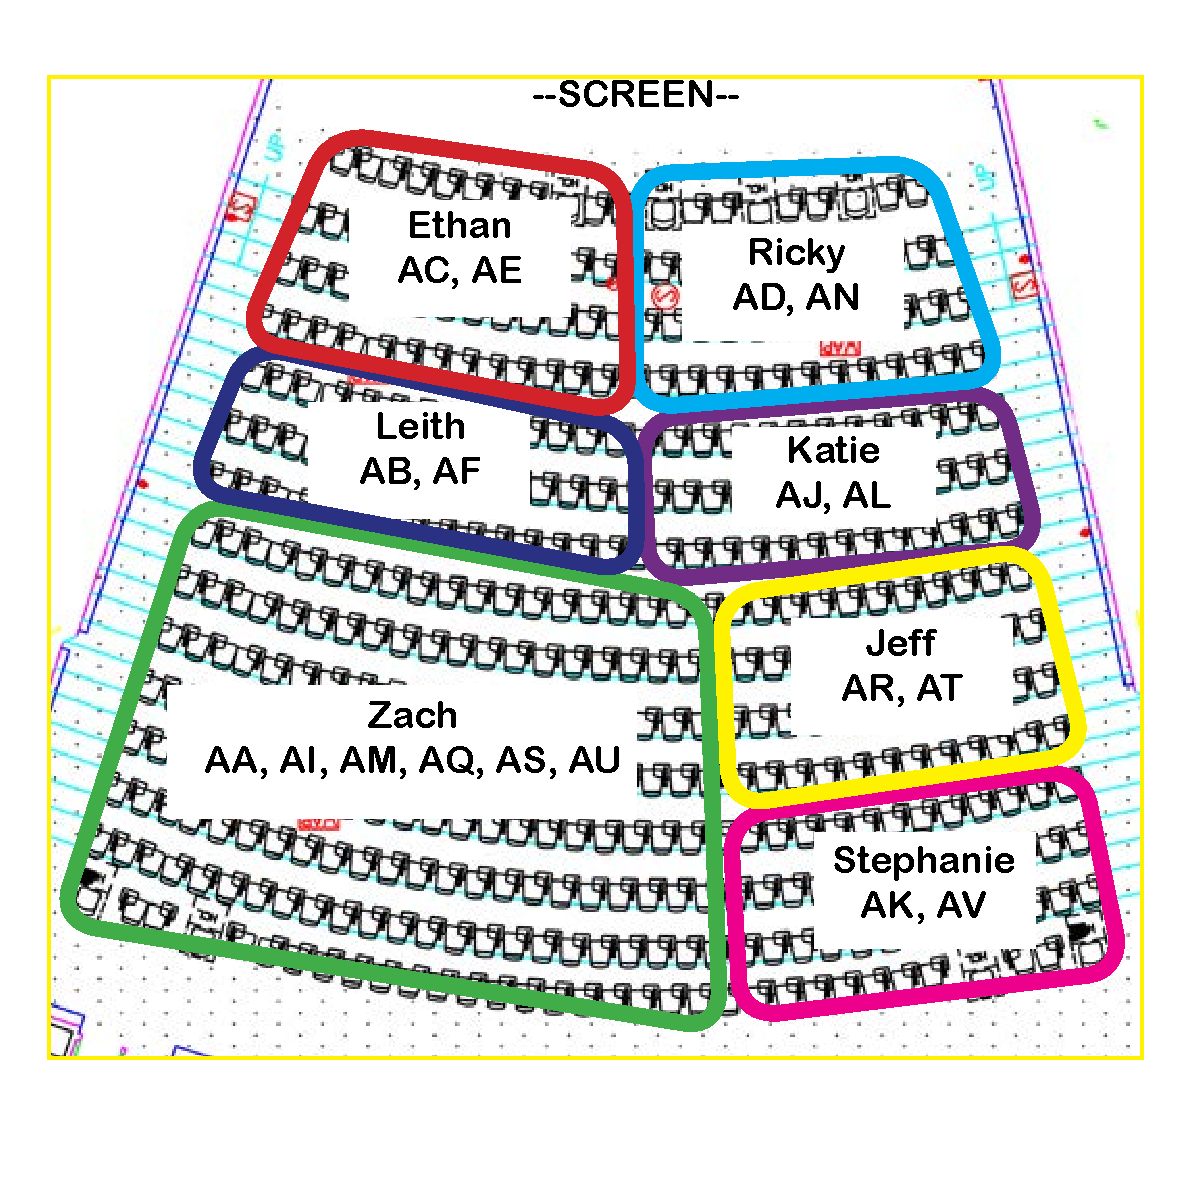
\includegraphics[height=1.3\textheight]{../images/seating-chart.pdf}
    \end{center}
\end{frame}
\end{noheadline}
}

\begin{noheadline}
\begin{frame}
\frametitle{Today's issues:}
\textbf{At the molecular level, what is a gene? An allele? A mutation?} \\
\vspace{5mm}
\tableofcontents[subsectionstyle=hide]
\end{frame}
\end{noheadline}

\section{The molecular nature of the gene}

\begin{frame}[t]
    What is the current definition of a gene?
    \uncover<2->{\footnote{\tiny We're not really sure.}}

    \nbox{A simple question, but turns out to be a very complicated answer.
        For BIO 180: A section of DNA that influences the phenotype for a
        particular trait.}
\end{frame}

\tikzstyle{nuc} = [
    minimum width=2.3ex, minimum height=2.3ex, node distance=2.3ex]
\tikzstyle{space} = []
    minimum width=2.3ex, minimum height=1ex, node distance=1ex]

\begin{frame}[t]
    \frametitle{What are genes made of?}
    \begin{adjustwidth}{-1.5em}{-1.5em}
    \centering{
        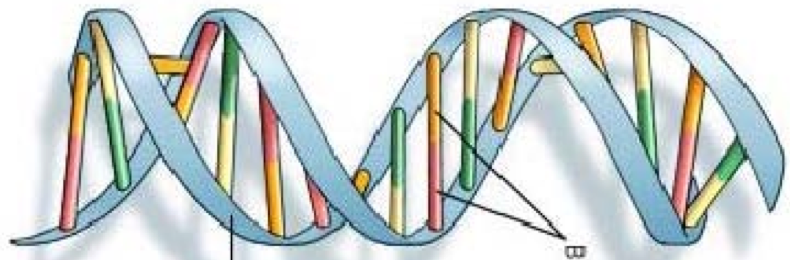
\includegraphics[width=0.5\linewidth]{dna-crop.png}
    }
    \begin{center}
    \begin{tikzpicture}[font=\sffamily]
        \node[visible on=<2->, name=tn1, nuc] {A};
        \node[visible on=<2->, name=tn2, nuc, right of=tn1] {T};
        \node[visible on=<2->, name=tn3, nuc, right of=tn2] {G};
        \node[visible on=<2->, name=tn4, nuc, right of=tn3] {T};
        \node[visible on=<2->, name=tn5, nuc, right of=tn4] {T};
        \node[visible on=<2->, name=tn6, nuc, right of=tn5] {A};
        \node[visible on=<2->, name=tn7, nuc, right of=tn6] {A};
        \node[visible on=<2->, name=tn8, nuc, right of=tn7] {G};
        \node[visible on=<2->, name=tn9, nuc, right of=tn8] {T};
        \node[visible on=<2->, name=tn10, nuc, right of=tn9] {G};
        \node[visible on=<2->, name=tn11, nuc, right of=tn10] {A};
        \node[visible on=<2->, name=tn12, nuc, right of=tn11] {G};
        \node[visible on=<2->, name=tn13, nuc, right of=tn12] {G};
        \node[visible on=<2->, name=tn14, nuc, right of=tn13] {C};
        \node[visible on=<2->, name=tn15, nuc, right of=tn14] {T};
        \node[visible on=<2->, name=tn16, nuc, right of=tn15] {A};
        \node[visible on=<2->, name=tn17, nuc, right of=tn16] {A};
        \node[visible on=<2->, name=tn18, nuc, right of=tn17] {T};
        \node[visible on=<2->, name=tn19, nuc, right of=tn18] {A};
        \node[visible on=<2->, name=tn20, nuc, right of=tn19] {G};

        \node[visible on=<2->, name=sn1, nuc, below of=tn1] {};
        \node[visible on=<2->, name=sn2, nuc, below of=tn2] {};
        \node[visible on=<2->, name=sn3, nuc, below of=tn3] {};
        \node[visible on=<2->, name=sn4, nuc, below of=tn4] {};
        \node[visible on=<2->, name=sn5, nuc, below of=tn5] {};
        \node[visible on=<2->, name=sn6, nuc, below of=tn6] {};
        \node[visible on=<2->, name=sn7, nuc, below of=tn7] {};
        \node[visible on=<2->, name=sn8, nuc, below of=tn8] {};
        \node[visible on=<2->, name=sn9, nuc, below of=tn9] {};
        \node[visible on=<2->, name=sn10, nuc, below of=tn10] {};
        \node[visible on=<2->, name=sn11, nuc, below of=tn11] {};
        \node[visible on=<2->, name=sn12, nuc, below of=tn12] {};
        \node[visible on=<2->, name=sn13, nuc, below of=tn13] {};
        \node[visible on=<2->, name=sn14, nuc, below of=tn14] {};
        \node[visible on=<2->, name=sn15, nuc, below of=tn15] {};
        \node[visible on=<2->, name=sn16, nuc, below of=tn16] {};
        \node[visible on=<2->, name=sn17, nuc, below of=tn17] {};
        \node[visible on=<2->, name=sn18, nuc, below of=tn18] {};
        \node[visible on=<2->, name=sn19, nuc, below of=tn19] {};
        \node[visible on=<2->, name=sn20, nuc, below of=tn20] {};

        \node[visible on=<2->, name=bn1, nuc, below of=sn1] {T};
        \node[visible on=<2->, name=bn2, nuc, below of=sn2] {A};
        \node[visible on=<2->, name=bn3, nuc, below of=sn3] {C};
        \node[visible on=<2->, name=bn4, nuc, below of=sn4] {A};
        \node[visible on=<2->, name=bn5, nuc, below of=sn5] {A};
        \node[visible on=<2->, name=bn6, nuc, below of=sn6] {T};
        \node[visible on=<2->, name=bn7, nuc, below of=sn7] {T};
        \node[visible on=<2->, name=bn8, nuc, below of=sn8] {C};
        \node[visible on=<2->, name=bn9, nuc, below of=sn9] {A};
        \node[visible on=<2->, name=bn10, nuc, below of=sn10] {C};
        \node[visible on=<2->, name=bn11, nuc, below of=sn11] {T};
        \node[visible on=<2->, name=bn12, nuc, below of=sn12] {C};
        \node[visible on=<2->, name=bn13, nuc, below of=sn13] {C};
        \node[visible on=<2->, name=bn14, nuc, below of=sn14] {G};
        \node[visible on=<2->, name=bn15, nuc, below of=sn15] {A};
        \node[visible on=<2->, name=bn16, nuc, below of=sn16] {T};
        \node[visible on=<2->, name=bn17, nuc, below of=sn17] {T};
        \node[visible on=<2->, name=bn18, nuc, below of=sn18] {A};
        \node[visible on=<2->, name=bn19, nuc, below of=sn19] {T};
        \node[visible on=<2->, name=bn20, nuc, below of=sn20] {C};

        \path[-] (tn1) edge [visible on=<2->, thick] (bn1);
        \path[-] (tn2) edge [visible on=<2->, thick] (bn2);
        \path[-] (tn3) edge [visible on=<2->, thick] (bn3);
        \path[-] (tn4) edge [visible on=<2->, thick] (bn4);
        \path[-] (tn5) edge [visible on=<2->, thick] (bn5);
        \path[-] (tn6) edge [visible on=<2->, thick] (bn6);
        \path[-] (tn7) edge [visible on=<2->, thick] (bn7);
        \path[-] (tn8) edge [visible on=<2->, thick] (bn8);
        \path[-] (tn9) edge [visible on=<2->, thick] (bn9);
        \path[-] (tn10) edge [visible on=<2->, thick] (bn10);
        \path[-] (tn11) edge [visible on=<2->, thick] (bn11);
        \path[-] (tn12) edge [visible on=<2->, thick] (bn12);
        \path[-] (tn13) edge [visible on=<2->, thick] (bn13);
        \path[-] (tn14) edge [visible on=<2->, thick] (bn14);
        \path[-] (tn15) edge [visible on=<2->, thick] (bn15);
        \path[-] (tn16) edge [visible on=<2->, thick] (bn16);
        \path[-] (tn17) edge [visible on=<2->, thick] (bn17);
        \path[-] (tn18) edge [visible on=<2->, thick] (bn18);
        \path[-] (tn19) edge [visible on=<2->, thick] (bn19);
        \path[-] (tn20) edge [visible on=<2->, thick] (bn20);
    \end{tikzpicture}
    \end{center}
    \begin{itemize}
        \item What do the ``bars'' in the cartoon, and the letters below
            represent?
            \nbox{The bars and letters both represent nucleotides (or
                bases)---the building block of DNA}

        \item Do you notice any patterns in the 2 rows of letters?
            \nbox{A's pair with T's; G's pair with C's (= complementary base
                pairing)}

        \item What does a chromosome consist of?
            \nbox{One long DNA molecule (a ``double helix'') (in some species,
                like eukaryotes, it is wrapped around proteins)}
    \end{itemize}

    \end{adjustwidth}
\end{frame}

\begin{frame}[t]
    \begin{adjustwidth}{-1.5em}{-1.5em}
    Why is it significant that in some parts of some genes, groups of 3 bases
    code for an amino acid?

    \vspace{5mm}
    \centering{
        
\includegraphics[width=\linewidth]{codons.png}
    }

    \nbox{Some genes code for proteins. Amino acids are the building blocks of
        proteins, which form structures and act as ``machines'' of the cell.
        DNA stores the information (code) for building and running cells.}
    \end{adjustwidth}
\end{frame}

\begin{frame}[t]
    \begin{adjustwidth}{-1.5em}{-1.5em}
    Different sections of a gene are referred to as \highlight{structural} or
    \highlight{regulatory}. What's the difference?

    \vspace{5mm}
    \centering{
        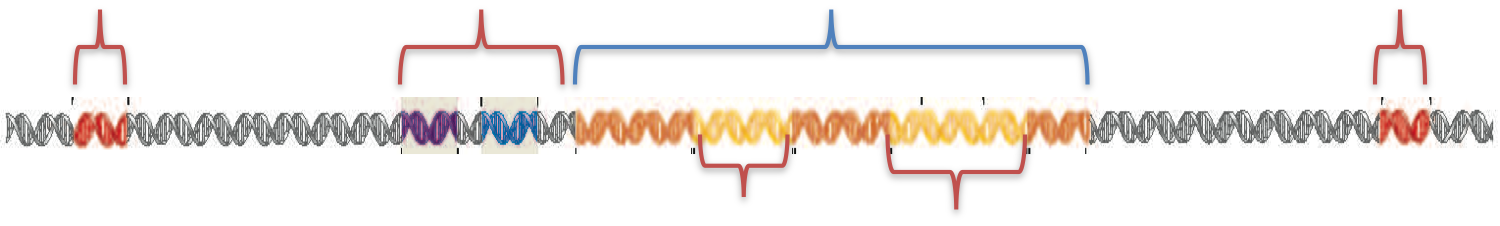
\includegraphics[width=\linewidth]{gene-regions.png}
    }

    \nbox{Structural regions code for an RNA or protein that functions in the
        cell; regulatory regions are responsible for controlling the
        \highlight{expression} of the gene (i.e., on/off/more/less).}
    \end{adjustwidth}
\end{frame}

\begin{frame}[t]
    \frametitle{The importance of regulatory sequences}
    \begin{adjustwidth}{-1.5em}{-1.5em}
    \begin{itemize}
        \item Muscle cells and nerve cells contain the same chromosomes. Why
            are the cells so different?

            \nbox{They express different genes at different times and in
                different quantities; this leads to different structure and
                function}

        \item Dr.\ Oaks has the genes required to make a uterus. Why doesn't he
            have one?

            \nbox{The genes responsible for the uterus never got turned on}

        \item In many cases, the proteins produced by homologous genes in
            chimps and humans are identical or nearly identical. Why are the
            two species so different?

            \nbox{There are differences in the regulatory sequences so that the
                timing and amount of expression of the proteins is different}
    \end{itemize}
    \end{adjustwidth}
\end{frame}

\section{The central dogma of molecular biology}

\begin{frame}
    \frametitle{The central dogma of molecular biology}
    \begin{adjustwidth}{-1.5em}{-1.5em}
    \begin{columns}
        \column{0.45\linewidth}
        
        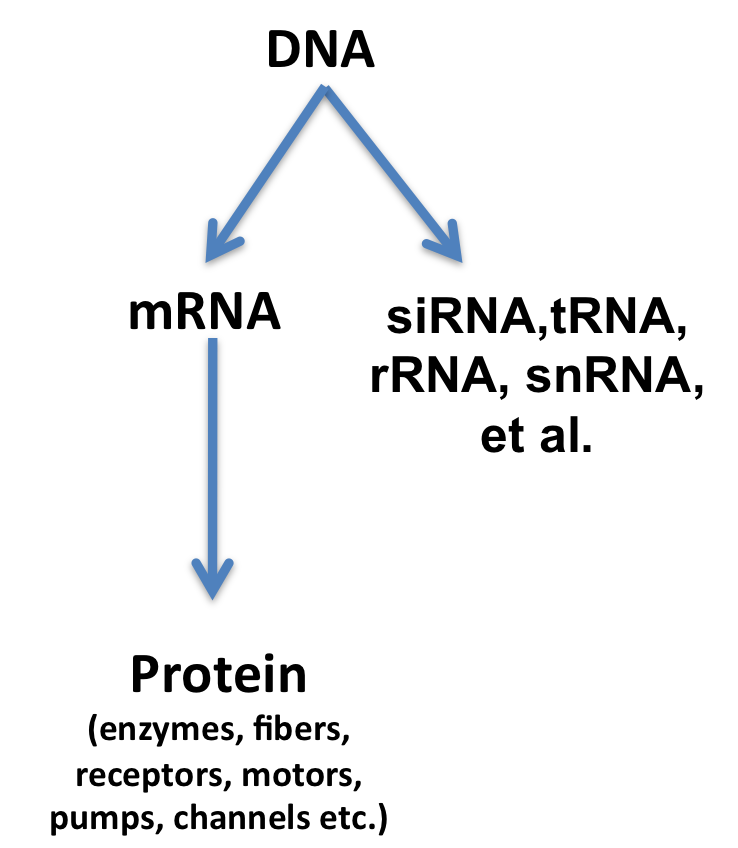
\includegraphics[width=\textwidth]{central-dogma.png}

        \column{0.55\linewidth}

        \uncover<2->{
        \begin{itemize}
            \item What do these arrows represent?
                \nbox{Enzyme-catalyzed reactions: Chemical reactions are making
                    new molecules from information coded in the DNA/RNA, and
                    these reactions are catalyzed by enzymes.}
            
            \item What makes up the genotype?

                \nbox{The sequence of bases in DNA; different sequences are
                    different alleles}

            \item What makes up the phenotype?

                \nbox{RNA and protein products}
        \end{itemize}
        }

    \end{columns}
    \end{adjustwidth}
\end{frame}

\begin{frame}[t]
    \begin{adjustwidth}{-1.5em}{-1.5em}
        \begin{itemize}
            \item At the molecular level, what is the ``gene for flower
                color?''

                \nbox{A DNA sequence (section of a chromosome) that codes for a
                    product that affects flower color.}

                \vspace{8mm}
            \item At the molecular level, what is an allele?

                \nbox{Any version of a gene that differs in DNA sequence.}

                \vspace{1.2cm}
            \item Often in the media you will hear, ``scientists discovered the
                gene for \underline{\ \ \ \ \ }.'' What is wrong with this?

                \nbox{It's almost always a new \highlight{allele} that is
                    found.}
        \end{itemize}
    \end{adjustwidth}
\end{frame}

\section{The molecular nature of mutation}


\end{document}


\clickerslide{
\begin{frame}
    \begin{clickerquestion}
        \item 
        \begin{clickeroptions}
            \item 
            \item 
            \item 
            \item 
        \end{clickeroptions}
    \end{clickerquestion}
\end{frame}
}
